%% -*- mode: latex; mode:flyspell -*-
\documentclass[svgnames,x11names]{beamer}

\usepackage[british]{babel}

\usepackage{minted,tikz,tcolorbox,calc,siunitx}
\usetikzlibrary{chains,positioning,shapes.geometric,shapes.symbols,calc,shadows}
\usetikzlibrary{circuits.ee.IEC}
\usepackage{pgfplots}
\usepackage{booktabs,inconsolata}


\title{Basic Electronics}
\subtitle{CM0506 -- Small Embedded Systems}
\date{Lecture 2}
\author{Dr Alun Moon}
\institute[CSDT]{Department of Computer Science and Digital Technology}

\definecolor{NUblue}{RGB}{62,141,165}
\definecolor{NUbluedark}{RGB}{40,119,143}

\usetheme{CambridgeUS}

\usecolortheme{crane}
\setbeamercolor*{palette primary}{use=structure,fg=white,bg=NUblue}
\setbeamercolor*{palette quaternary}{fg=white,bg=NUbluedark}
\setbeamercolor{section in head/foot}{fg=white,bg=NUbluedark}
\setbeamercolor{subsection in head/foot}{fg=white,bg=NUblue}
\setbeamercolor{frametitle}{fg=NUbluedark!150,bg=NUblue!40}
\setbeamercolor{title in head/foot}{fg=white,bg=NUblue}
\setbeamercolor{author in head/foot}{fg=white, bg=NUbluedark}
\setbeamercolor{date in head/foot}{fg=white, bg=NUblue!60}
\setbeamercolor{title}{fg=NUbluedark!150,bg=NUblue!30}
\setbeamercolor{date}{fg=NUbluedark!150}
\setbeamercolor{block title}{fg=white,bg=NUblue}

\usepackage[T1]{fontenc}
\usepackage[utf8]{inputenc}


\begin{document}

\frame\maketitle

\begin{frame}{Energy}
  \begin{description}
  \item[Energy] is work done (force $\times$ distance)
    \begin{itemize}
    \item 1 Joule (\si\joule) = 1 Newton (\si\newton) $\times$ 1
      metre (\si\meter)
    \end{itemize}
  \item[Power] is rate of work, energy transfer
    \begin{itemize}
    \item Power = Energy/time
    \item 1 Watt (\si\watt) = 1 Joule / 1 second
    \item 1 Joule = 1 Watt $\times$ 1 second
    \end{itemize}
  \end{description}
\end{frame}

\begin{frame}{Electrical Energy}
  \begin{itemize}
  \item Electrical power = Voltage $\times$ Current
    \begin{itemize}
    \item 1 Watt = 1 Volt $\times$ 1 Ampere
      (\SI{1}{\watt}=\SI{1}{V}$\times$\SI{1}{A})
    \item $P = VI$
    \end{itemize}
  \item 1 Joule = 1 Watt $\times$ 1 second
  \item 1 Joule = 1 Volt $\times$ 1 Ampere $\times$ 1 second
  \item House meter measures units of electrical energy
    \begin{itemize}
    \item \SI{1}{\kilo\watt\hour} = \SI{1000}{W}$\times$\SI{1}{\hour}
      = \SI{3600000}{\joule}
    \end{itemize}

  \end{itemize}
\end{frame}

\begin{frame}{Charge}
\begin{itemize}
\item Charge is a state of matter (like temperature,
colour, density \ldots)
\item Electron is the smallest negatively charged particle
\item Proton is the smallest positively charged particle
\item An uncharged object/body has equal number of
electrons and protons in all its constituent atoms  
\end{itemize}
\end{frame}

\begin{frame}{Charge}
  \begin{itemize}
  \item \alert{Only electrons} can leave the owning nucleus of the atom
  \item \alert{Absence of electrons} results in positive charge
  \item Materials in which electrons can easily leave nuclei are
    called \break \alert{electrical conductors}
    \begin{itemize}
    \item copper
    \item aluminium
    \item silver
    \item gold
    \end{itemize}
  \item Materials in which electrons are tightly bound to their nuclei
    are called \alert{electrical insulators}
    \begin{itemize}
    \item rubber
    \item mica
    \item bakelite
    \end{itemize}
  \end{itemize}
\end{frame}

\begin{frame}{Charge}
  \begin{itemize}
  \item Electrical charge is measured in Coulombs \si\coulomb
  \item 1 Coulomb = \num{6.3e18} electrons
  \item So 1 e = \num{1.602e-19} Coulomb
  \end{itemize}
\end{frame}

\begin{frame}{Current}
  \begin{itemize}
  \item An electrical current is flow of charge past across a point
    over a period of time
  \item 1 Ampere = 1 Coulomb/second
  \item (\SI{300}{mA} through your body can be fatal)
  \item Electron current -- the actual movement of electrons
  \item Conventional current $I$ -- (opposite to electron flow)
    \begin{itemize}
    \item flows from positive to negative
    \item shows by arrows in symbols for diodes \tikz[circuit ee
      IEC,set diode graphic=var diode IEC graphic]\draw (0,0) to
      [diode] (1,0);
    \end{itemize}
  \end{itemize}
\end{frame}

\begin{frame}{Voltage or Potential Difference}
  \begin{itemize}
  \item It is the \alert{electrical force} that can
    \begin{itemize}
    \item push/pull charge
    \item cause charge to move/flow
    \end{itemize}
  \item 1 Volt = 1 Joule / Coulomb
  \item Constant voltage
    \begin{itemize}
    \item  Battery cell \SI{1.5}{\volt}
    \item `square' battery \SI{9}{\volt}
    \end{itemize}
  \item  time-varying voltage
    \begin{itemize}
    \item UK houses are supplied with time-varying voltage of
      nominal value \SIrange{230}{240}{V} (US \SI{110}{V})
    \end{itemize}
  \end{itemize}
\end{frame}

\begin{frame}{Voltage}
  \begin{itemize}
  \item Voltage comes \alert{before} current
  \item Voltage across two ends of a conductor can cause a current
  \end{itemize}
  \begin{columns}[onlytextwidth]
    \begin{column}{0.4\textwidth}
      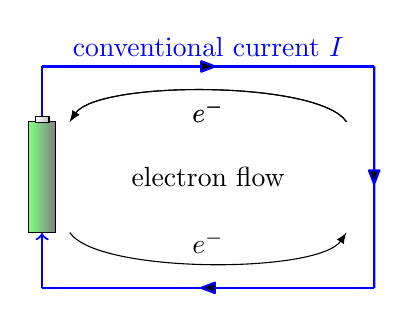
\begin{tikzpicture}[x=1em,y=1em,circuit ee IEC]
        \node[rectangle,draw,inner sep=0pt,
              minimum width=10pt,minimum height=40pt,
              left color=green!50,right color=black!50]
              (batt){};
        \node[rectangle,draw,inner sep=0pt,
              minimum width=5pt,minimum height=2pt,
              left color=white,right color=Silver,
              above=-0.5pt of batt](term){};
        \begin{scope}[thick,blue]
          \draw (term.north) -- (0,4);
          \draw (0,4) to[current direction]
           node[above,sloped]{conventional current $I$} (12,4) ; 
          \draw (12,4) to[current direction] (12,-4);
          \draw (12,-4) to[current direction] (0,-4);
          \draw[->] (0,-4) --
          (batt.south);
        \end{scope}
        \begin{scope}
          \draw[latex-] (1,2) .. controls (2,3.5) and (10,3.5) ..
          node[below]{$e^-$} (11,2); \draw[-latex] (1,-2) .. controls
          (2,-3.5) and (10,-3.5) ..  node[above]{$e^-$} (11,-2);
          \draw[latex-] (1,2) .. controls (2,3.5) and (10,3.5) ..
          node[below]{$e^-$} (11,2);
        \end{scope}
          \node at (6,0) {electron flow};
      \end{tikzpicture}
    \end{column}
    \begin{column}{0.5\textwidth}
      \begin{eqnarray*}
        V &=& IR \\
&\text{so}\\ 
        I &=& \frac{V}{R}
      \end{eqnarray*}
      Low resistance $\rightarrow$ high current
    \end{column}
  \end{columns}
  \begin{alertblock}{}
    \alert{don't!} Short-circuit
  \end{alertblock}
  
\end{frame}

\begin{frame}{Resistance}
  \begin{itemize}
  \item Electrical appliances transform electrical energy into other
    forms
    \begin{itemize}
    \item lightbulb
    \item fan
    \item radio
    \item cooker
    \end{itemize}

  \item Electrical appliances (and all materials) have
    \alert{electrical resistance}:
    \begin{block}{}
      ``resistance to (flow of) electrical current''
    \end{block}
  \item Unit is \alert{Ohm} symbol \si{\ohm}
  \item 1 ohm = 1Volt/1Ampere
  \end{itemize}
\end{frame}

\begin{frame}{Resistance}
  \begin{itemize}
  \item \SI{50}{\ohm} is less resistance than \SI{500}{\ohm}
  \item A resistance is better than a bare wire (short circuit)
  \item Still think!  Check the expected current!
  \end{itemize}
  \begin{columns}[onlytextwidth]
    \begin{column}{0.35\textwidth}
      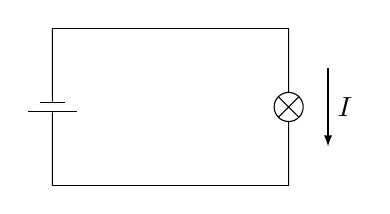
\begin{tikzpicture}[circuit ee IEC]
        \node[coordinate] (bl) at (0,0) {};
        \node[coordinate] (tl) at (0,2) {};
        \node[coordinate] (tr) at (3,2) {};
        \node[coordinate] (br) at (3,0) {};

        \draw (bl) to [battery] (tl);
        \draw (tl) -- (tr) (br) -- (bl);
        
        \draw (tr) to [bulb] (br);
    
        \draw[-latex] ($(tr)+(0.5,-0.5)$) -- node[right] {$I$} ($(br)+(0.5,0.5)$);
      \end{tikzpicture}
    \end{column}
    \begin{column}{0.2\textwidth}
      \begin{eqnarray*}
        I &=& \frac{V}{R}
      \end{eqnarray*}
    \end{column}
    \begin{column}{0.3\textwidth}
      For a \SI{1.5}{V} battery
      \begin{tabular}{rr}\toprule
        resistance & current \\\midrule
        \SI{50}{\ohm} & \SI{50}{\milli\ampere}\\
        \SI{500}{\ohm} & \SI{5}{\milli\ampere}\\
      \end{tabular}
    \end{column}
  \end{columns}
  \begin{block}{}
    normal circuit
  \end{block}
\end{frame}

\begin{frame}{Resistance}{Open circuit}
  \begin{itemize}
  \item Break in connection
  \item $R = \infty $
  \end{itemize}
  \begin{columns}[onlytextwidth]
    \begin{column}{0.33\textwidth}
      \begin{tikzpicture}[circuit ee IEC]
        \node[coordinate] (bl) at (0,0) {};
        \node[coordinate] (tl) at (0,2) {};
        \node[coordinate] (tr) at (3,2) {};
        \node[coordinate] (br) at (3,0) {};

        \draw (bl) to [battery] (tl);
        \draw (tl) -- (tr) (br) -- (bl);
        
        \draw (tr) -- ($(tr)!.3!(br)$) ($(tr)!.7!(br)$) -- (br);
    
      \end{tikzpicture}
    \end{column}
    \begin{column}{0.66\textwidth}
      \begin{eqnarray*}
      I &=& \frac{V}{R} \\
      \therefore  I &=& 0
    \end{eqnarray*}
  \end{column}
  \end{columns}
\end{frame}

\begin{frame}{Resistance}{Short circuit}
  \begin{itemize}
  \item conducting connection
  \item $R = 0 $
  \end{itemize}
  \begin{columns}[onlytextwidth]
    \begin{column}{0.33\textwidth}
      \begin{tikzpicture}[circuit ee IEC]
        \node[coordinate] (bl) at (0,0) {};
        \node[coordinate] (tl) at (0,2) {};
        \node[coordinate] (tr) at (3,2) {};
        \node[coordinate] (br) at (3,0) {};

        \draw (bl) to [battery] (tl);
        \draw (tl) -- (tr) (br) -- (bl);
        
        \draw (tr) -- (br);
    
      \end{tikzpicture}
    \end{column}
    \begin{column}{0.66\textwidth}
      \begin{eqnarray*}
      I &=& \frac{V}{R} \\
      \therefore  I &=& \infty
    \end{eqnarray*}
    \end{column}
  \end{columns}
\end{frame}

\begin{frame}
  \frametitle{Ohm's Law}
  \begin{block}{Ohm's law} states that the current through a conductor between two
    points is directly proportional to the potential difference across
    the two points.
    \[ V = IR \hspace{5em} I=\frac{V}{R} \hspace{5em} R=\frac{V}{I} \]
  \end{block}

\end{frame}

\begin{frame}
  \frametitle{Ohm's Law}
  \framesubtitle{$I = V/R $}
  \begin{columns}[onlytextwidth]
    \begin{column}{0.33\textwidth}
      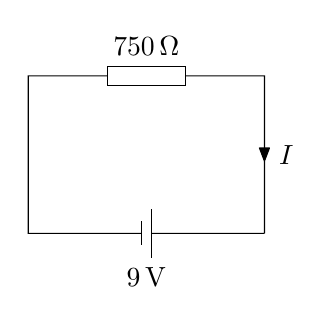
\begin{tikzpicture}[circuit ee IEC]
        \node[coordinate] (bl) at (0,0) {};
        \node[coordinate] (tl) at (0,2) {};
        \node[coordinate] (tr) at (3,2) {};
        \node[coordinate] (br) at (3,0) {};

        \draw (br) to[battery={info={\SI{9}{\volt}}}] (bl) -- (tl) 
        to [resistor={info={\SI{750}{\ohm}}}] (tr) 
        to [current direction={info={$I$}}] (br);
      \end{tikzpicture}
    \end{column}
    \begin{column}{0.66\textwidth}
      \[
      I = \frac{9}{750} = \SI{0.012}{\ampere} = \SI{12}{\milli\ampere}
      \]
    \end{column}
  \end{columns}  
\end{frame}

\begin{frame}
  \frametitle{Ohm's Law}
  \framesubtitle{$V = IR$}
  \begin{center}
    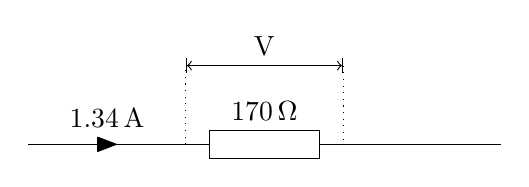
\begin{tikzpicture}[circuit ee IEC,huge circuit symbols]
      \draw (0,0) to [current direction={info={\SI{1.34}{\ampere}}}]
      (2,0) to [resistor={info={\SI{170}{\ohm}}}] (4,0) -- (6,0);
      \draw[|<->|](2,1)--node[above]{\si{\volt}}(4,1); \draw[dotted]
      (2,0)--(2,1) (4,1)--(4,0);
    \end{tikzpicture}
  \end{center}
      \[
      V = 1.34\times 170 = \SI{227.8}{\volt}
      \]
\end{frame}

\begin{frame}
  \frametitle{Ohm's Law}
  \framesubtitle{$R = V/I$}
  \begin{columns}[onlytextwidth]
    \begin{column}{0.33\textwidth}
      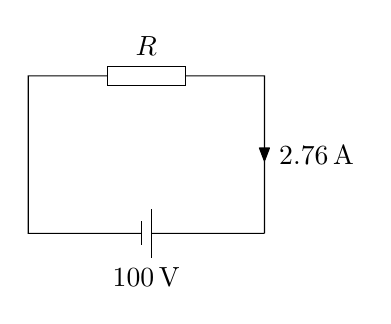
\begin{tikzpicture}[circuit ee IEC]
        \node[coordinate] (bl) at (0,0) {};
        \node[coordinate] (tl) at (0,2) {};
        \node[coordinate] (tr) at (3,2) {};
        \node[coordinate] (br) at (3,0) {};

        \draw (br) to[battery={info={\SI{100}{\volt}}}] (bl) -- (tl) 
        to [resistor={info={$R$}}] (tr) 
        to [current direction={info={\SI{2.76}{\ampere}}}] (br);
      \end{tikzpicture}
    \end{column}
    \begin{column}{0.66\textwidth}
      \[
      R = \frac{100}{2.76} = \SI{36.2}{\ohm}
      \]
    \end{column}
  \end{columns}  
\end{frame}

\begin{frame}
  \frametitle{Resistor Colour Coding}
  \begin{itemize}
  \item Carbon resistors -- small size -- hence coded
  \item Surface mount -- even smaller -- same scheme using small printing
\item
  \begin{tabular}{cccccccccc}
    Bk&Br&R&O&Y&Gn&Bu&V&Gy&W\\
    0&1&2&3&4&5&6&7&8&9
  \end{tabular}
\item Tolerance
  \begin{description}
  \item[Gold] 5\%
  \item[Silver] 10\%
  \end{description}
\end{itemize}
\end{frame}

\begin{frame}
  \frametitle{Resistor Colour Coding}
  \begin{columns}[onlytextwidth]
    \begin{column}{.5\textwidth}
      Hold with bands at left \vspace{1em}

  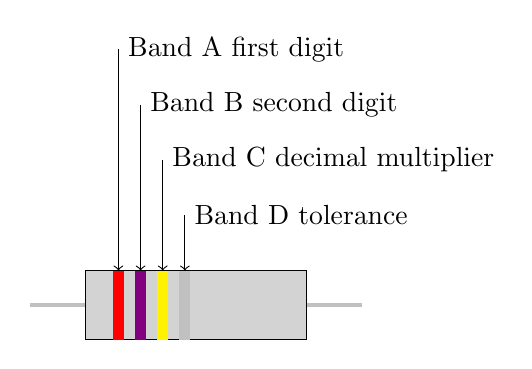
\begin{tikzpicture}[x=10pt,y=10pt]
    \draw[ultra thick,Silver] (0,0) -- (12,0);
    \draw[thin,fill=LightGray] (2,-1.25) rectangle (10,1.25);
    \path[fill=red] (3,-1.25) rectangle +(0.4,2.5); \path[fill=violet]
    (3.8,-1.25) rectangle +(0.4,2.5); \path[fill=yellow] (4.6,-1.25)
    rectangle +(0.4,2.5); \path[fill=Silver] (5.4,-1.25) rectangle
    +(0.4,2.5);

    \draw[<-] (3.2,1.25) -- +(0,8) node[right] {Band A \alert{first
        digit}}; \draw[<-] (4.0,1.25) -- +(0,6) node[right] {Band B
      \alert{second digit}}; \draw[<-] (4.8,1.25) -- +(0,4)
    node[right] {Band C \alert{decimal multiplier}}; \draw[<-]
    (5.6,1.25) -- +(0,2) node[right] {Band D \alert{tolerance}};
  \end{tikzpicture} 
\end{column}
\begin{column}{.45\textwidth}
  \begin{tabular}{cccc}
  Red & Violet & Yellow & Silver \\
  2 & 7 & 4 & 10\% \\
  2 & 7 & $\times 10^4$ & $\pm 10\%$
\end{tabular}
\\[1ex]
Resistance is \SI{270000}{\ohm} or \SI{270}{\kilo\ohm}\\
Value may be between\\
\hfil \SI{243}{k\ohm} and \SI{297}{k\ohm}
\end{column}
\end{columns}
\end{frame}

\begin{frame}
  \frametitle{Series Circuits}
  \begin{itemize}
  \item Same current in \alert{all} parts
  \item Total resistance is sum of all resistances
  \item Series $IR$ drops the sum of voltage drops
  \end{itemize}

  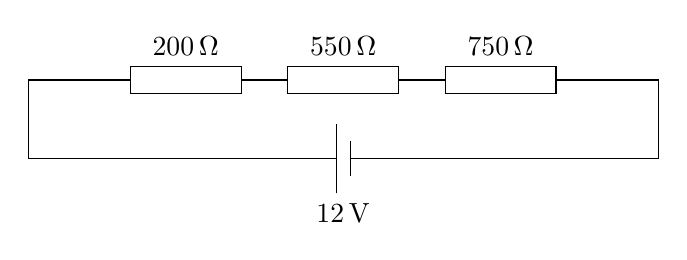
\begin{tikzpicture}[circuit ee IEC,huge circuit symbols]
    \draw (0,0) -- ++(up:1) -- ++(right:1)
          to[resistor={info=\SI{200}{\ohm}}] ++(right:2)
          to[resistor={info=\SI{550}{\ohm}}] ++(right:2)
          to[resistor={info=\SI{750}{\ohm}}] ++(right:2)
          -- ++(right:1) -- ++(down:1) node[coordinate](a){};
    \draw (0,0) to[battery={info'={\SI{12}{\volt}}}] (a);
  \end{tikzpicture}
\[
I = \frac{V}{R}= \frac{V}{\sum R} = \frac{12}{200+550+750} =
\frac{12}{1500} = \SI{8}{\milli\ampere}
\]
\end{frame}
\begin{frame}
  \frametitle{Parallel Circuits}
  \begin{itemize}
  \item Applied voltage is the same across all branches
  \item Each branch current is $V_A/R$
  \item Current draw $I_T$ is sum of branch currents
  \end{itemize}

  \begin{columns}[onlytextwidth]
    \begin{column}{0.5\textwidth}
  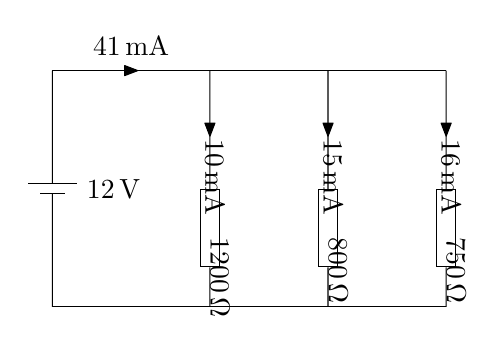
\begin{tikzpicture}[circuit ee IEC]
    \draw (0,0) to[battery={info={\SI{12}{V}}}] (0,-3);
    \draw (0,0)
          to[current direction={info={\SI{41}{\milli\ampere}}}]
          (2,0)--
          (5,0);
    \draw (5,-3) -- (0,-3);
    \foreach \position/\current/\resistance in {2/10/1200,3.5/15/800,5/16/750}
    {
      \draw (\position,0) 
          to[current direction={
            near end,info sloped={\SI{\current}{\milli\ampere}}}]
          ++(down:1)
          to[resistor={info sloped={\SI{\resistance}{\ohm}}}] ++(down:2);
        }
  \end{tikzpicture}
\end{column}
    \begin{column}{0.5\textwidth}
      \begin{eqnarray*}
        I_1&=&\frac{12}{1200}=\SI{10}{\milli\ampere}\\
        I_2&=&\frac{12}{ 800}=\SI{15}{\milli\ampere}\\
        I_3&=&\frac{12}{ 750}=\SI{16}{\milli\ampere}\\
        I_T &=&  10+15+16 = 41
      \end{eqnarray*}
\end{column}
\end{columns}
\end{frame}
\begin{frame}
  \frametitle{Kirchoff's Laws}
  \framesubtitle{Continuity laws}
  \begin{itemize}
  \item Similar to conservation of mass and energy laws
  \item Charge is conserved (mass)
  \item Voltage is conserved (energy)
  \end{itemize}
  \begin{block}{Kirchoff’s Current Law}
    The algebraic sum of all currents entering and
leaving any point in a circuit must equal zero
  \end{block}
  \begin{block}{Kirchoff’s Voltage Law}
    For any loop or closed path in a circuit, the algebraic sum 
    of voltages must equal zero
  \end{block}
\end{frame}

\begin{frame}
  \frametitle{Kirchoff’s Current Law}
  \begin{itemize}
  \item The algebraic sum of all currents entering and leaving any
    point in a circuit must equal zero
  \item Currents entering and leaving a node are equal
  \end{itemize}
  \begin{columns}[onlytextwidth]
    \begin{column}{0.5\textwidth}
  \[ I_1 = I_2 + I_3 \]
\end{column}
    \begin{column}{0.5\textwidth}
\begin{tikzpicture}[circuit ee IEC]
    \node (in) at (left:2) {$I_1$};
    \node (out 1) at (60:2) {$I_2$};
    \node (out 2) at (-60:2) {$I_3$};
    \node[contact] at (0,0){};
    \draw (in) to[current direction] (0,0);
    \draw (0,0) to[current direction] (out 1);
    \draw (0,0) to[current direction] (out 2);
  \end{tikzpicture}
\end{column}
\end{columns}
\end{frame}

\begin{frame}\frametitle{Kirchoff’s Voltage Law}
  \begin{itemize}
  \item For any loop or closed path in a circuit, the algebraic sum
    of voltages must equal zero
  \item The sum of voltage sources must equal the sum of voltage drops
    around the loop
  \end{itemize}
  \begin{columns}[onlytextwidth]
    \begin{column}{0.5\textwidth}
      \[ V = I_1 R_1 + I_2 R_2 \]
    \end{column}
    \begin{column}{0.5\textwidth}
      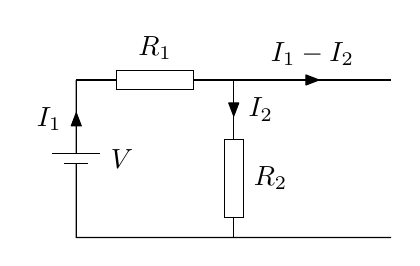
\begin{tikzpicture}[circuit ee IEC]
        \draw (0,0) to[
        current direction'={near start,info={$I_1$}},
        battery={info={$V$}}
        ] (down:2) -- ++(right:4);
        \draw (0,0) to[resistor={info={$R_1$}}] (2,0)
        to[
        current direction={info={$I_2$},near end}]
        (2,-0.5)
        to[
        resistor={info={$R_2$}}
        ]
        (2,-2);
        \draw (2,0) to[current direction={info={$I_1-I_2$}}] (4,0);
      \end{tikzpicture}
    \end{column}
  \end{columns}
\end{frame}

\begin{frame}
  \frametitle{AC/DC or AV/DV ? }
  \begin{itemize}
  \item Remember voltage comes first
  \item Direct Voltage $\rightarrow$ Direct Current
  \item Alternating Voltage $\rightarrow$ Alternating Current
  \item DC implies DV
  \item AC implies AV
  \item DV should be called Constant Voltage: does not vary with time
    say \SI{+12}{\volt} or \SI{-5}{\volt}
  \item Measured with respect to ‘ground’ i.e. \SI{0.0}{V}
  \end{itemize}
\end{frame}

\begin{frame}
  \frametitle{DC (DV)}
  \begin{tikzpicture}
    \begin{axis}[width=\textwidth,height=\textheight,domain=0:10,
                 xmax=10.5,,xlabel={time},
                 ymin=-15,ymax=16,ylabel={voltage},
                 axis x line=middle,axis y line=left]
      \addplot+[no marks,thick]{12};
      \addplot+[no marks,thick]{-5};
    \end{axis}
  \end{tikzpicture}
\end{frame}

\begin{frame}
  \frametitle{Time Varying Voltage}
  \begin{tikzpicture}
    \begin{axis}[width=\textwidth,height=\textheight,domain=0:10,
                 xmax=10.5,,xlabel={time},
                 ymin=-15,ymax=16,ylabel={voltage},
                 axis x line=middle,axis y line=left]
      \addplot[blue,no marks,thick] coordinates {(0,0) (2,10)};
      \addplot[blue,no marks,smooth,thick] coordinates 
      {(2,10) (4,5) (6,15) (10,10)};
    \end{axis}
  \end{tikzpicture}
\end{frame}

\begin{frame}
  \frametitle{Alternating Periodic Voltage}
  \begin{tikzpicture}
    \begin{axis}[width=\textwidth,height=\textheight,domain=0:10,
                 xmax=10.5,,xlabel={time},
                 ymin=-15,ymax=16,ylabel={voltage},
                 axis x line=middle,axis y line=left]
      \addplot+[no marks,thick] coordinates {(0,0) (1.5,10) (3,0) (4.5,-10)
        (6,0) (7.5,10) (9,0) (10.5,-10)};
    \end{axis}
  \end{tikzpicture}
\end{frame}

\begin{frame}
  \frametitle{Clock signal}
  \begin{tikzpicture}
    \begin{axis}[width=\textwidth,height=0.7\textheight,domain=0:10,
                 xmax=65,xlabel={time/\si{\milli\second}},
                 ymin=-5,ymax=11,ylabel={voltage/\si{\volt}},
                 axis x line=middle,axis y line=left]
      \addplot+[no marks,const plot,thick] coordinates {
        (0,5) (10,0) (20,5) (30,0) (40,5) (50,0) (60,5)
      };
    \end{axis}
  \end{tikzpicture}
\end{frame}

\begin{frame}
  \frametitle{Square wave}
  \begin{tikzpicture}
    \begin{axis}[width=\textwidth,height=0.7\textheight,domain=0:10,
                 xmax=65,xlabel={time/\si{\milli\second}},
                 ymin=-110,ymax=110,ylabel={voltage/\si{\milli\volt}},
                 axis x line=middle,axis y line=left]
      \addplot+[no marks,const plot,thick] coordinates {
        (0,50) (10,-50) (20,50) (30,-50) (40,50) (50,-50) (60,50)
      };
    \end{axis}
  \end{tikzpicture}
\end{frame}

\begin{frame}
  \frametitle{UK Mains Voltage}
  \framesubtitle{\SI{230}{\volt}pp \SI{50}{\hertz} AC}
  \begin{tikzpicture}
    \begin{axis}[width=\textwidth,height=0.8\textheight,
                 domain=0:60,samples=60,
                 xmax=65,xlabel={time/\si{\milli\second}},
                 ymin=-350,ymax=350,ylabel={voltage/\si{\volt}},
                 axis x line=middle,axis y line=left]
      \addplot+[no marks,smooth,thick] {330*sin(x*18)};
      \addplot[dotted]{230} node {\small \SI{230}{\volt}RMS};
      \addplot[dotted]{-230};
    \end{axis}
  \end{tikzpicture}
\end{frame}

\begin{frame}
  \frametitle{Sine wave -- safe}
  \framesubtitle{\SI{\pm 15}{\volt} \SI{50}{\hertz} AC}
  \begin{tikzpicture}
    \begin{axis}[width=\textwidth,height=0.8\textheight,
                 domain=0:60,samples=60,
                 xmax=65,xlabel={time/\si{\milli\second}},
                 ymin=-20,ymax=20,ylabel={voltage/\si{\volt}},
                 axis x line=middle,axis y line=left]
      \addplot+[no marks,smooth,thick] {15*sin(x*18)};
      \addplot[dotted]{230} node {\small \SI{230}{\volt}RMS};
      \addplot[dotted]{-230};
    \end{axis}
  \end{tikzpicture}
\end{frame}

\begin{frame}
  \frametitle{Wavelength, Bandwidth}
  \begin{itemize}
  \item Electromagnetic waves are sinusoids that travel with speed of
    light  $c=\SI{3e8}{\meter\per\second}$
  \item  for waves
    \begin{itemize}
    \item velocity = frequency \emph{times} wavelength
      \[ v = f\lambda \]
    \item Say $f = \SI{2}{\mega\hertz}$ (million cycles per sec)
    \item then wavelength $\lambda = 300000000/2000000 = \SI{150}{\meter}$
    \end{itemize}

  \item Bandwidth refers to a range of
    frequencies
    \begin{itemize}
    \item e.g FM radio: \SI{88}{\mega\hertz} -- \SI{108}{\mega\hertz}
    \item so bandwidth = \SI{20}{\mega\hertz}
    \end{itemize}
  \end{itemize}
\end{frame}

\begin{frame}
  \frametitle{Notable frequency ranges}
  \begin{description}
  \item[Human speech] \SI{100}{\hertz} to \SI{7000}{\hertz}
  \item[Intelligent part (voice band)] \SI{300}{\hertz} to \SI{3400}{\hertz}
  \item[Telephone] \SI{250}{\hertz} to \SI{3500}{\hertz}
  \item[Audible] \SI{20}{\hertz}  to \SI{20000}{\hertz}
  \item[In music]:
    \begin{description}
    \item[low frequencies] Bass
    \item[high frequencies] Treble
    \end{description}

  \end{description}
\end{frame}
    
% \begin{frame}{References}
% Electronics for Beginners at
% \url{http://library.thinkquest.org/16497/home/index.html}
% \end{frame}

%%%% --------
\end{document}
